% Generated from the Notion page by tools/notion2tex.py (see report/README.md).
\section{Agent-Driven Design Space Exploration}\label{sec:3}

\subsection{Why an agent}\label{sec:3.1}

Optimizing an HLS accelerator is a search. Every iteration follows the same fixed loop: choose one optimization, change the code, run C simulation, run HLS synthesis, read the reports, and, for promising candidates, run C/RTL co-simulation and Vivado place-and-route. The loop is slow (one synthesis of this design takes 10 to 60 minutes on our host and one implementation up to three hours), the reports are long, and the space of techniques is large: precision, tiling, line buffers, loop pipelining and unrolling, dataflow, DSP packing, Winograd, parameter storage, FIFO depths and clock targets can be combined in countless ways. As beginners without hardware intuition we could not pick the right combination directly, and we could not afford to try many combinations by hand.

Both Vitis HLS and Vivado expose complete command-line flows, so the loop can be driven by a program. We therefore handed the loop to general-purpose LLM coding agents (OpenAI Codex and Anthropic Claude Code) running on a laptop and executing the tools over SSH on a Linux host (12 logical CPUs, 15 GiB of memory) with the Xilinx installation. This section describes how the agents were controlled, what the resulting search looked like, what the method caught that we would otherwise have missed, and which decisions were made by humans. The hardware results themselves are analyzed in Section~\ref{sec:4}.

\subsection{The problem was not the model}\label{sec:3.2}

Our first attempts showed that a capable model is not enough. Left alone, an agent tends to:

\begin{itemize}
\item change several things at once, so that a measured gain cannot be attributed to any one of them;
\item explain results after the fact, adjusting its expectation to whatever the tool reported;
\item present a weaker result as a stronger one, for example reporting an HLS latency estimate as if it were the frame time, or a functional pass as a speedup;
\item lose track of what has already been tried over a session that lasts many hours.
\end{itemize}

None of these are failures of hardware knowledge. They are failures of experimental discipline, and they are the same failures a student makes. Mature frameworks now exist for constraining a model and automating its workflow. Building on Claude Code, we wrote the discipline down as a rules file (\texttt{AGENTS.md}) and a reusable skill file that the agent loads at the start of every session; Figure~\ref{fig:1} shows an excerpt. The rest of this section is that method.

\begin{figure}[!htbp]
\centering
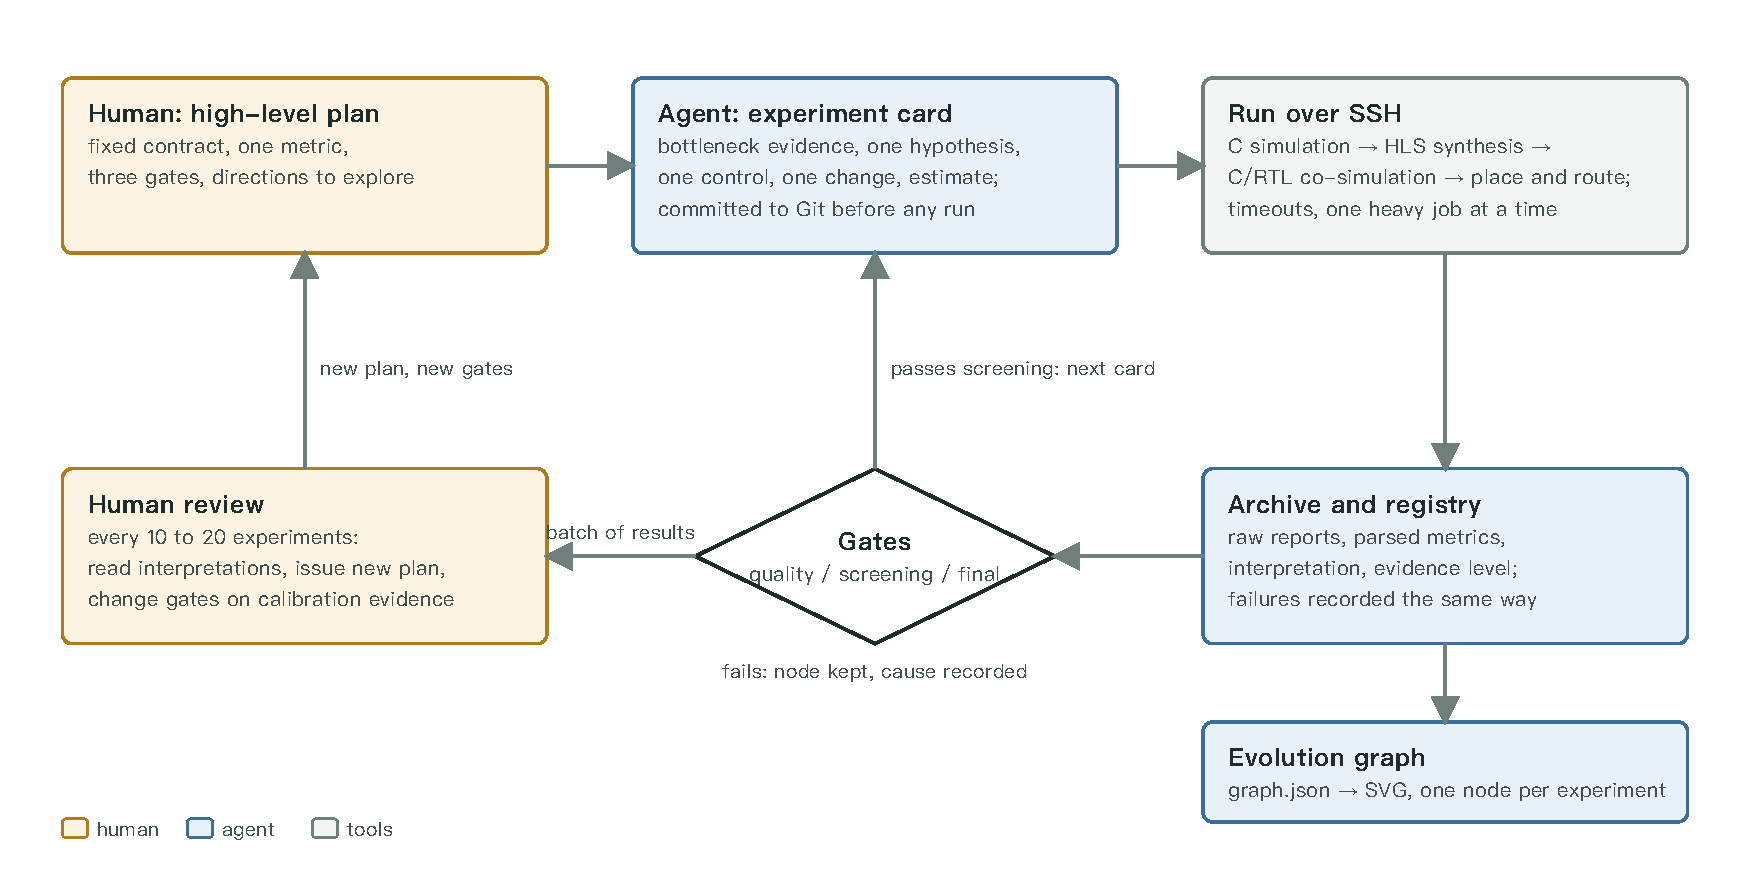
\includegraphics[width=0.9\figw]{figures/fig01-experiment-loop.pdf}
\caption{Excerpt of the rules file (AGENTS.md) loaded by the coding agent at the start of every session, which fixes the experimental discipline described in this section.}
\label{fig:1}
\end{figure}

\subsection{The protocol}\label{sec:3.3}

\textbf{Plan before experimenting.} Planning happens at two levels. A high-level plan (\texttt{docs/\allowbreak{}000N-*.md}) fixes what must not change, what is being optimized, and which directions to explore. For this project the fixed contract is: the \texttt{srcnn} function signature with float arrays, runtime-loaded parameters, replicate padding, the 1-64-32-1 network, and bit-exact agreement with a fixed-point reference on all 13 Set14 images. The single primary metric is milliseconds per frame, computed as cycles multiplied by clock period. Three gates separate ``ran'' from ``counts''; they are defined in Table~\ref{tab:2}.

\begin{table}[!htbp]
\centering
\footnotesize
\caption{The three acceptance gates of the exploration protocol and the concrete criterion used for each in this project.}
\label{tab:2}
\begin{tabularx}{\linewidth}{lp{3.4cm}Y}
\toprule
Gate & Question & Criterion used in this project \\
\midrule
Quality & Is the output correct? & Bit-exact against the 10-bit \texttt{ap\_fixed} reference E017 (or the mixed-precision reference E065) on every image; mean PSNR change on Set14 no worse than -0.1 dB \\
Screening & Is it worth verifying further? & HLS synthesis completes with II = 1 in the compute loops and resources inside an explicit screen (for the T4 designs: DSP $\le$ 1100, LUT $\le$ 170 k, FF $\le$ 230 k) \\
Final & Can we call it feasible? & Post-route timing met at the implemented clock, zero unrouted nets, routed resources within the device, and C/RTL co-simulation bit-exact over two or more frames with finite FIFOs \\
\bottomrule
\end{tabularx}
\end{table}

Only designs that pass the final gate enter the ranking. We review the completed experiments and issue a new high-level plan; the agent does not change the gates itself.

\textbf{Register before running.} Every experiment gets an immutable ID (E, P, W, G, S, C, F series by direction) and a card that is committed to Git before any tool runs. The card contains the bottleneck evidence (a specific line of a specific report), one hypothesis, one control experiment, the single thing changed relative to the control, and a paper estimate of DSP, BRAM, LUT, FF and cycles with its derivation. Because the card is committed first, the estimate cannot be adjusted afterwards. Listing~\ref{lst:1} shows the relevant part of one card.

\begin{lstlisting}[caption={Experiment card C13 (excerpt), planned 2026-10-12T04:58 UTC, control W21.},label={lst:1},language={}]
Change: T=4 fold; Conv2 only switches to E065's signed 8-bit weights, two coefficients
        pre-packed per 27-bit DSP operand once per frame; everything else frozen.
Paper estimate: DSP 1032 (576+256+200), BRAM18K 146, LUT 150000, FF 220000,
        latency 292000 cycles.  Basis: 2304/4 Conv1, 2048/(4*2) Conv2 pairs, 800/4 Conv3;
        C11 measured 1036 DSP / 198436 LUT / 231297 FF with the old loader.
Measured (HLS): DSP 1032, BRAM18K 146, LUT 127966 (-14.7 %), FF 192308 (-12.6 %),
        263090 cycles (-9.9 %).  All deviations within 20 %.
\end{lstlisting}

\textbf{Record everything, with an evidence level.} Each run is archived under \texttt{experiments/\allowbreak{}<ID>\_\allowbreak{}<name>/\allowbreak{}} with the card, the source snapshot, the raw logs, the parsed reports and a one-page interpretation. Failed, timed-out and invalid runs are archived in the same way; 100 of the 231 registered experiments ended in \texttt{fail}, \texttt{infeasible}, \texttt{invalid\_config} or \texttt{timeout}. The registry \texttt{results.csv} is generated by a parser from the reports and is never edited by hand. Every number carries its evidence level, in increasing order of strength:

\begin{quote}
paper estimate $\rightarrow$ C simulation $\rightarrow$ HLS synthesis estimate $\rightarrow$ C/RTL co-simulation $\rightarrow$ post-route implementation $\rightarrow$ on-board measurement
\end{quote}

The agent may not present a lower level as a higher one. The log records the rule being applied: ``a functional PASS is not a speedup'' (F45), ``a slack-derived period is not a verified clock'' (W22), ``the clock and the thread count changed together, so the runtime change cannot be credited to threads''. In practice this rule is what forced us to notice that HLS estimates are systematically wrong for this design (see the decisions below).

\textbf{Draw the evolution graph and hand over.} Later experiments build on the results or hypotheses of earlier ones, so the experiments form a directed graph. The agent maintains \texttt{graph.json} with one node per experiment and one edge per dependency (design lineage, retry after fix, integration, numerical evidence, control, verification), and a script renders it. At the end of each session a progress file records the current branch, the running jobs, the open decisions and how to resume, so that a new session or a different model can continue without re-deriving the state.

\subsection{The search as a whole}\label{sec:3.4}

The agents registered 231 experiments over 71 design directories; the registry timestamps run from 2026-10-10 to 2026-10-13, with the baseline setup starting on 2026-09-29. 20 experiments reached Vivado implementation and 16 reached C/RTL co-simulation. Figure~\ref{fig:2} condenses the search to its 51 turning points; the complete graph and the per-route views are in the repository.

\begin{figure}[!htbp]
\centering
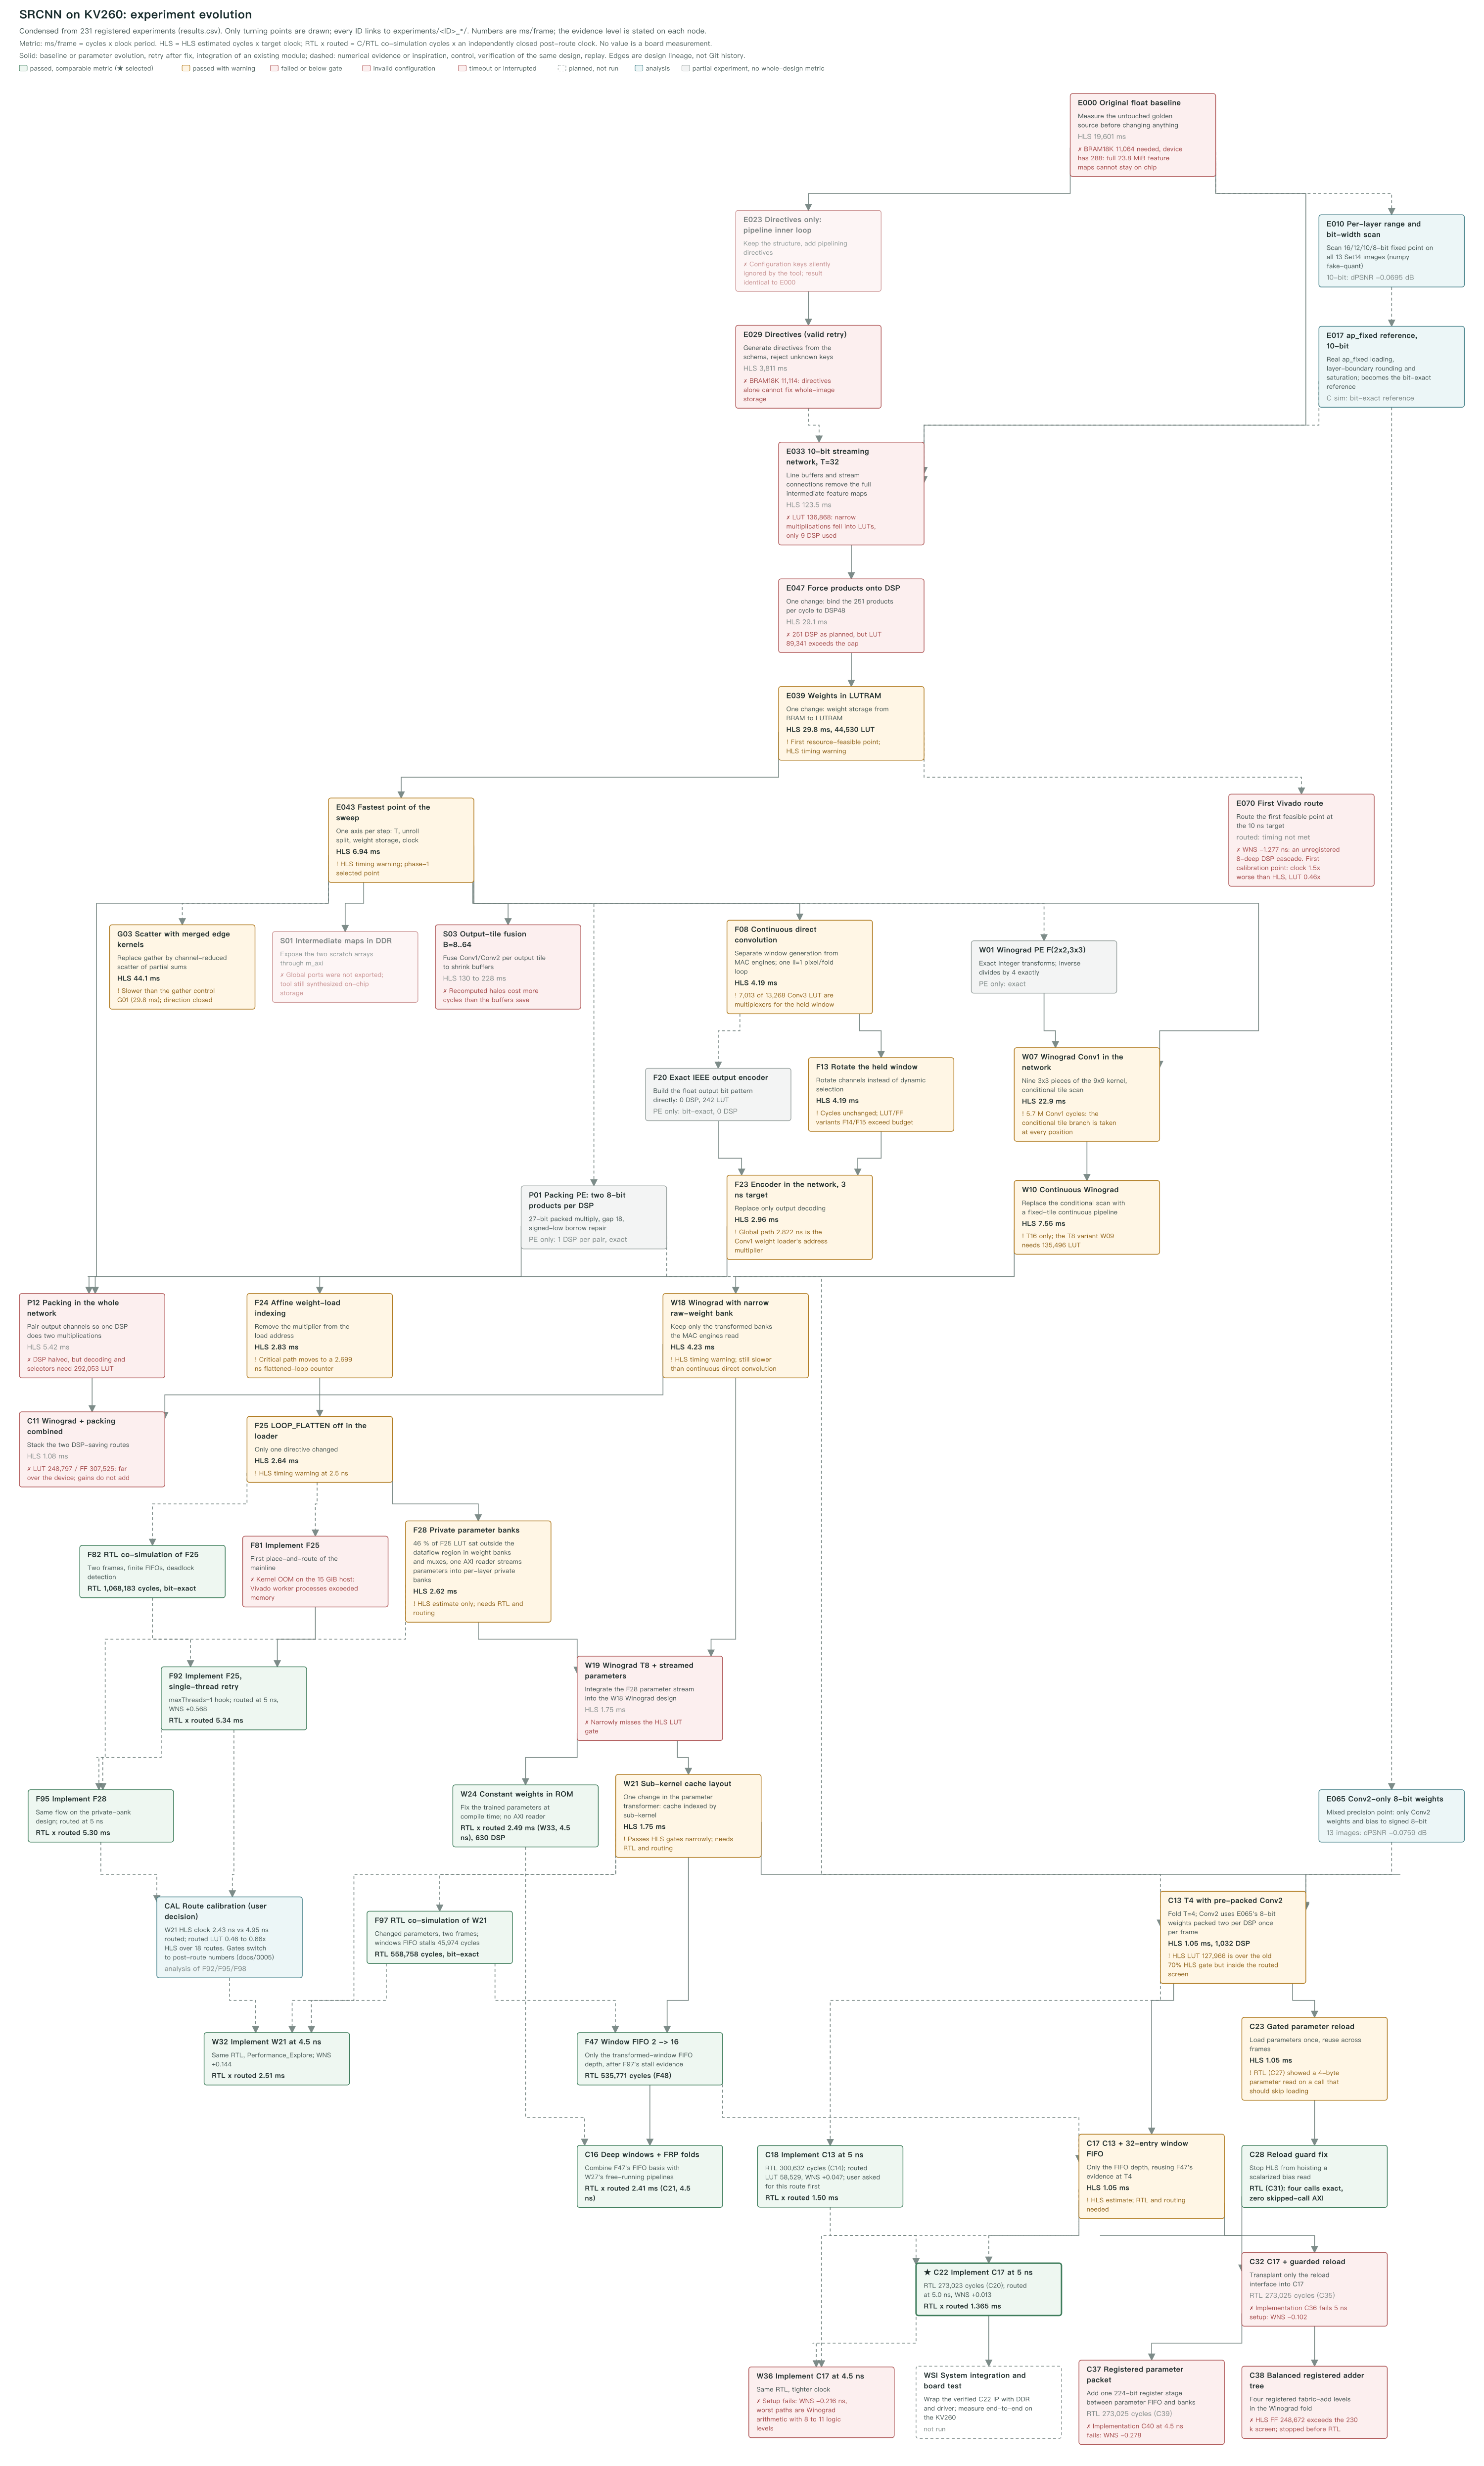
\includegraphics[width=\linewidth,height=0.95\figh,keepaspectratio]{figures/fig02-evolution-overview.png}
\caption{The search as a directed graph: 51 turning points out of 231 registered experiments. Solid edges are design lineage, dashed edges are evidence or verification; red nodes failed a gate, green nodes passed with a comparable number; the star marks the selected design C22.}
\label{fig:2}
\end{figure}

\subsection{Division of labour}\label{sec:3.5}

The agent did the mechanical and the clerical work: writing cards, copying and modifying designs, running the tools over SSH, parsing reports, updating the registry, drawing the graph, and drafting the interpretation of each run. It also proposed most of the individual experiments from the bottleneck evidence in the reports: the loader address multiplier in F23's timing report led to F24 and F25; the finding that 46 \% of F25's LUTs sat outside the dataflow region in weight banks and multiplexers led to the streamed-parameter designs F27 and F28; the FIFO stall profile of F97 led to F47.

We did the work that needs judgement about the goal rather than about the next step:

\begin{itemize}
\item writing and revising the high-level plans, and choosing which directions to pursue (Winograd and DSP packing were explored because the lectures covered them; the INT16 packing study P13 to P16 was requested by us);
\item changing the gates from HLS estimates to routed results on 2026-10-12 once the calibration data existed, and defining the 13 supplied images as the complete test set;
\item setting the host policy: how many jobs may run at once, the memory budget, enabling zram, and cleaning 55 GiB of old workspaces;
\item ordering priorities, for example asking for C18 to be routed before the planned T8 experiments, accepting F48 as the new T8 baseline, and declining a rescue re-route of C36 in favour of the verified C22;
\item reading every interpretation before the next plan was issued, roughly one review per 10 to 20 experiments.
\end{itemize}

Not every human decision was good. Our instruction to run two implementations at once caused the W23 out-of-memory failure; the one-heavy-job rule that replaced it came from the agent's measurement of the memory peaks.

\subsection{The directions we set}\label{sec:3.6}

In practice we set the following high-level directions, and the agent carried out the finer-grained implementation.

\begin{itemize}
\item \textbf{Fix the precision first, then work on the architecture.} The agent tried different precision requirements layer by layer, and in the first phase we settled on w10a10acc23 (10-bit weights, 10-bit activations, 23-bit accumulators), built a bit-exact \texttt{ap\_fixed} reference (E017, E019) and an exhaustive boundary check (E049). All two hundred or so later designs were required to match this reference bit for bit, so that every difference between experiments could be attributed to structure rather than to numerics. At the same time we explicitly rejected uniform INT8 (a 5.18 dB drop in mean PSNR on Set14) and admitted only 8-bit weights on Conv2 alone (E062, E065, a 0.0759 dB drop). This single exception later became the key to fitting the T4 design into the device.
\item \textbf{Abandon the directive-only route in the first phase.} E020 to E032 showed that the original code needs 11,064 BRAM18K no matter which pragmas are added. This negative result saved all later ``try one more pragma'' time and sent the search straight to a streaming architecture.
\item \textbf{Identify the weight-bank multiplexers as the real LUT bottleneck.} This was the most valuable single analysis of the whole trajectory (docs/0004 \S{}1.4). Breaking down the csynth report showed that 46 \% of the LUTs sat outside the dataflow region, in the multiplexers between the load loop and the engines across 324 to 648 LUTRAM banks. After F27 switched to streamed parameter loading, the out-of-region LUTs fell from 32 k to 3.2 k, and T8 became feasible.
\item \textbf{Judge feasibility by routed results, not HLS estimates.} This decision was made by us on 2026-10-12. The five calibration points available at the time all showed the HLS LUT estimate about 2$\times$ too high and the clock estimate about 2$\times$ too optimistic, and all 18 routed designs since have followed the same pattern. W21's HLS LUT count of 81,086 sat right at the threshold but routed to only 42.6 k; C13/C17 at 128 k HLS LUTs were ``infeasible'' under the old rule but routed to 59.5 k. Without this decision the T4 designs would never have been sent to place-and-route, and the 1.365 ms result would not exist. The companion decision was to stop tuning against the HLS clock estimate and look only at the routed critical path.
\item \textbf{Use Winograd only at T8/T4, not at T16.} At T16, W18 reduced the DSP count from 502 to 326 but left the cycle count unchanged, so there was no speed gain. Winograd only became useful once direct convolution at T8 needed 1,007 DSPs (81 \%) and Winograd brought that down to 648.
\item \textbf{Strict definitions of frame time and evidence level.} Only ``RTL cycles $\times$ closed clock'' counts; HLS estimates do not, and a period derived from negative WNS is treated as an estimate only. This prevented F25's 2.64 ms (at an estimated 2.5 ns) from being taken as a result; after routing it was 5.34 ms.
\item \textbf{Host resource management.} After three OOM kills we fell back to serial execution, then moved to ``one heavy job plus light jobs'' admitted under a memory budget, enabled zram, and cleaned 55 GiB of old workspaces. This is not a design decision, but it determined the experiment throughput.
\item \textbf{Three scope decisions.} The 13 supplied images are the complete test set; the interface may gain a \texttt{load\_params} switch; ROM parameter storage is exploratory only and does not enter the mainline. We made these three decisions on 12 and 13 October, and each one closed a bottomless pit.
\end{itemize}

\subsection{Limitations and lessons}\label{sec:3.7}

\begin{itemize}
\item \textbf{The method is expensive.} 231 experiments is far more than a human would run, and most of them are negative results or verification runs of the same design at another evidence level. The archive occupies several GB, the host ran continuously for three days, and the timeouts were 60 minutes for synthesis, 6 hours for co-simulation and 3 hours for implementation. The cost was worth paying only because each run is cheap to launch and the discipline makes negative results useful too.
\item \textbf{HLS estimates cannot be used for ranking.} For this design the HLS clock estimate is optimistic by 1.7 to 2$\times$ and the logic resource estimate pessimistic by about 2$\times$. Any search that ranks by HLS estimates would pick the wrong design. Routing is slow, so the compromise is to screen with HLS and rank only with routed numbers.
\item \textbf{The agent still needs a reviewer, and still makes mistakes.} The rules stop the agent from changing several things at once or overstating evidence, but they do not stop it from spending experiments on a direction that has stopped making sense; the review of the high-level plan is where that is corrected. The log also records clerical errors that the protocol caught after the fact: one experiment (W26) was launched before its design existed, one plan specified three co-simulation calls where four were needed, and a conditionally triggered implementation job was never started, leaving the host idle for several hours.
\item \textbf{The counts depend on the counting rules.} We count every registered run, including retries, controls and verification runs; there are 71 design directories, of which about 50 are distinct architectural points.
\item \textbf{No on-board feedback during the search.} All ranking during the search was based on RTL co-simulation and routed results; board integration was done only after the search ended. The gap between the on-board hardware time of 2.938 ms and the RTL $\times$ routed figure of 1.365 ms (166.665 MHz instead of 200 MHz, and single-beat AXI reads) was invisible at every evidence level available during the search, which shows that the top level of the evidence hierarchy cannot be skipped.
\end{itemize}
